\documentclass[12pt]{article}
\pagestyle{empty}
\usepackage{amsmath,times,bm,hyperref}
\usepackage{amssymb}
\usepackage{graphicx}
\usepackage{listings}
\usepackage{xcolor}
\lstset { %
    language=C++,
    backgroundcolor=\color{black!5}, % set backgroundcolor
    basicstyle=\footnotesize,% basic font setting
}

%%%%%%%%%%%%%%%%%%%%%%%%%%%%%%%%%%%%%%%%%%%%%%%%%%
% Do not modify the dimensions of the page
\setlength{\topmargin}{0mm}
\setlength{\headheight}{0mm}
\setlength{\headsep}{0mm}
%% 25.4 -25.4 = 0
\setlength{\topmargin}{0mm}
%% 25.4 -25.4 = 0
\setlength{\oddsidemargin}{0mm}
%% 210 -25(left) -25(right) = 160
\setlength{\textwidth}{160mm}
%% 297 -25(top) -30(bottom) = 242
\setlength{\textheight}{242mm}
\setlength{\parindent}{0pt}
\setlength{\parskip}{12pt}
% Do not modify the dimensions of the page
%%%%%%%%%%%%%%%%%%%%%%%%%%%%%%%%%%%%%%%%%%%%%%%%%%

\begin{document}

\begin{center}
% TITLE: replace text with your abstract title WITHOUT full stop
\textbf{\Large
Homework 2
}\\
\normalsize Due March 30 2021

% AUTHOR/AFFILIATION: handled by authblk. 
% Use only one of the two following methods for author listing. Delete or comment out the other.
% Add/remove authors/affiliations as necessary, complete following the template without adding additional superscript/footnotes  

% 1- Authors have the same affiliation:
% ~~~~~~~~~~~~~~~~~~~~~~~~~~~~~~~~~~~~


%%%%% AFFILIATIONS %%%%%

\end{center}
\begin{enumerate}
\item The three-point Gaussian quadrature is given as follows. The quadrature points are $-\sqrt{3/5}$, $0$, and $\sqrt{3/5}$; the corresponding quadrature weights are $5/9$, $8/9$, and $5/9$. Verify that its algebraic accuracy is $5$.

\item Consider the mesh shown in Figure \ref{fig:mesh}. Setup the IEN, ID, and LM arrays for this mesh. Notice that the essential boundary condition is specified on nodes 5, 6, 7, and 8.

\begin{figure}[h]
	\begin{center}
	\begin{tabular}{c}
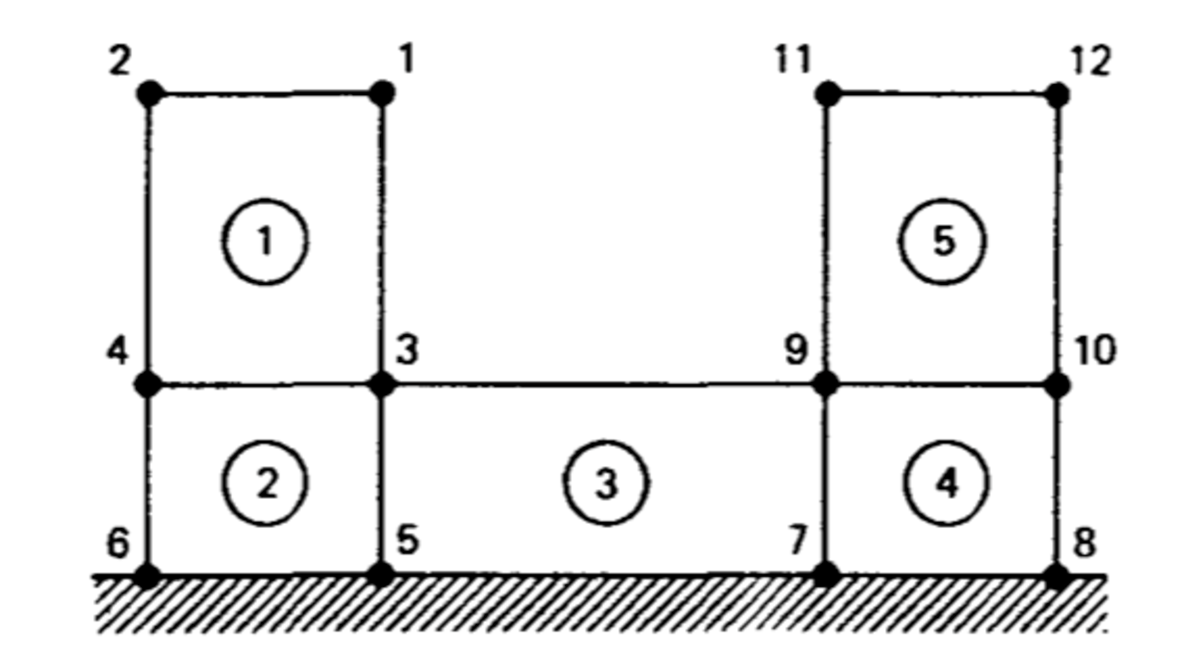
\includegraphics[angle=0, trim=0 0 0 0, clip=true, scale = 0.5]{./mesh-ien-id-lm.pdf}
\end{tabular}
\end{center} 
\caption{A finite element mesh consisting of five bilinear quadrilateral elements.}
\label{fig:mesh}
\end{figure}

\item Consider the 10-node tetrahedral element shown in Figure \ref{fig:tet10}. Derive the shape functions and verify that they satisfy the interpolation property, that is, $N_a(r_b, s_b, t_b, u_b) = \delta_{ab}$ with $u_b = 1 - r_b - s_b - t_b$.

\begin{figure}[h]
	\begin{center}
	\begin{tabular}{c}
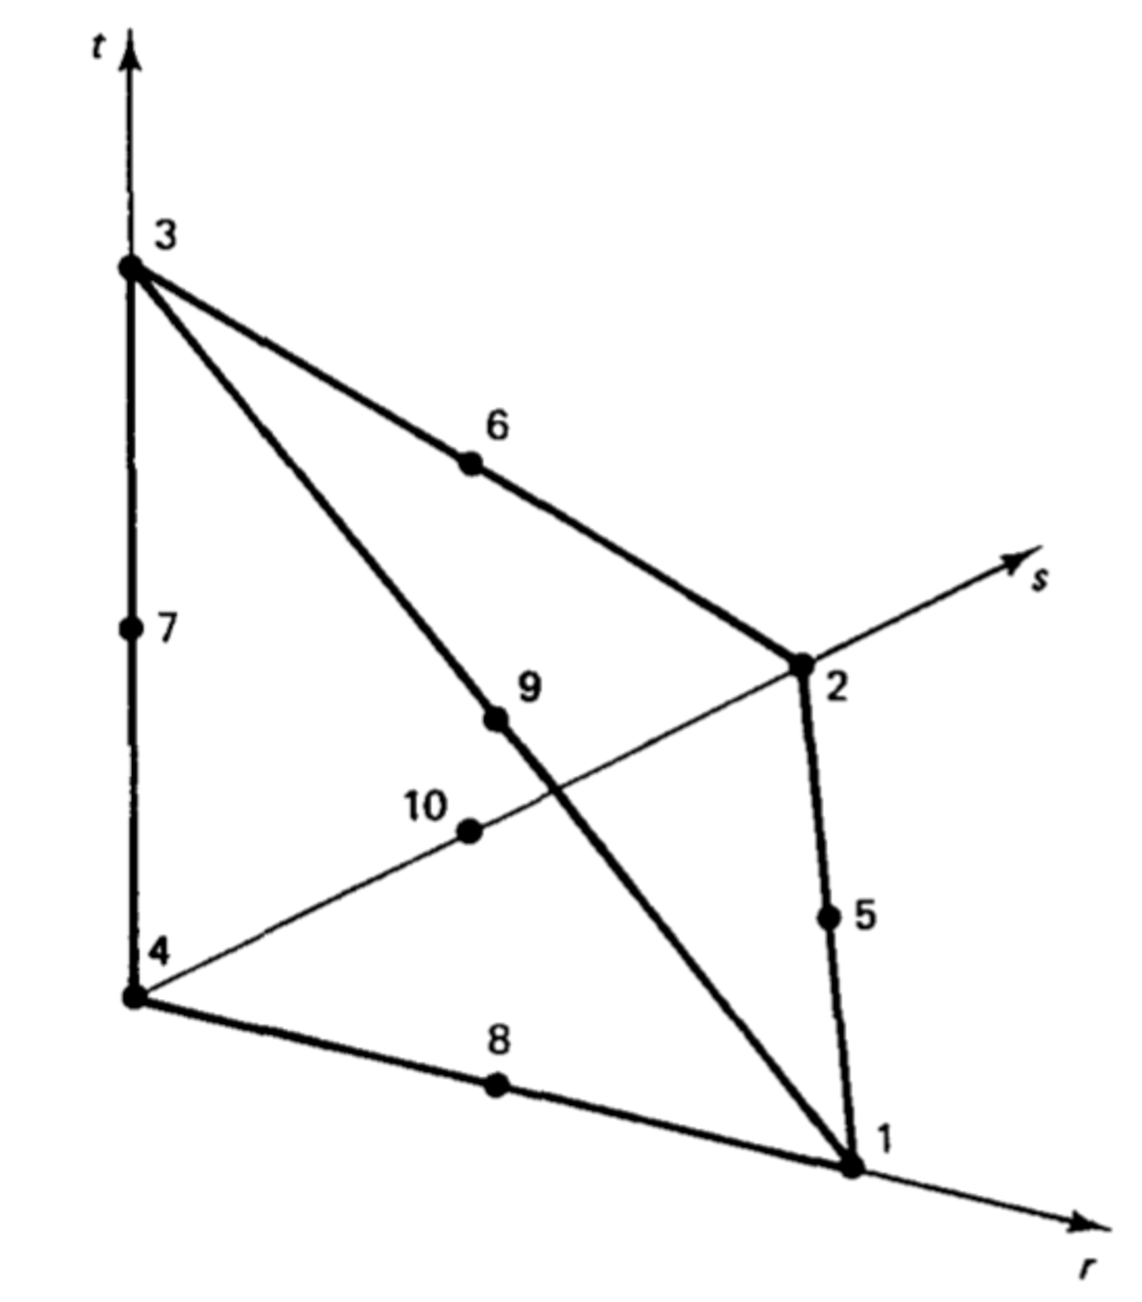
\includegraphics[angle=0, trim=0 0 0 0, clip=true, scale = 0.35]{./tet10.pdf}
\end{tabular}
\end{center} 
\caption{Quadratic tetrahedral element in the reference domain.}
\label{fig:tet10}
\end{figure}

\item Consider a one-dimensional quadratic three-node element shown in Figure \ref{fig:quad_elem}. The shape functions are given as follows.
\begin{align*}
N_1(\xi) = \frac12 \xi \left( \xi - 1 \right), \quad N_2(\xi) = 1 -\xi^2, \quad N_3(\xi) = \frac12 \xi \left( \xi + 1 \right).
\end{align*}

\begin{figure}[h]
	\begin{center}
	\begin{tabular}{c}
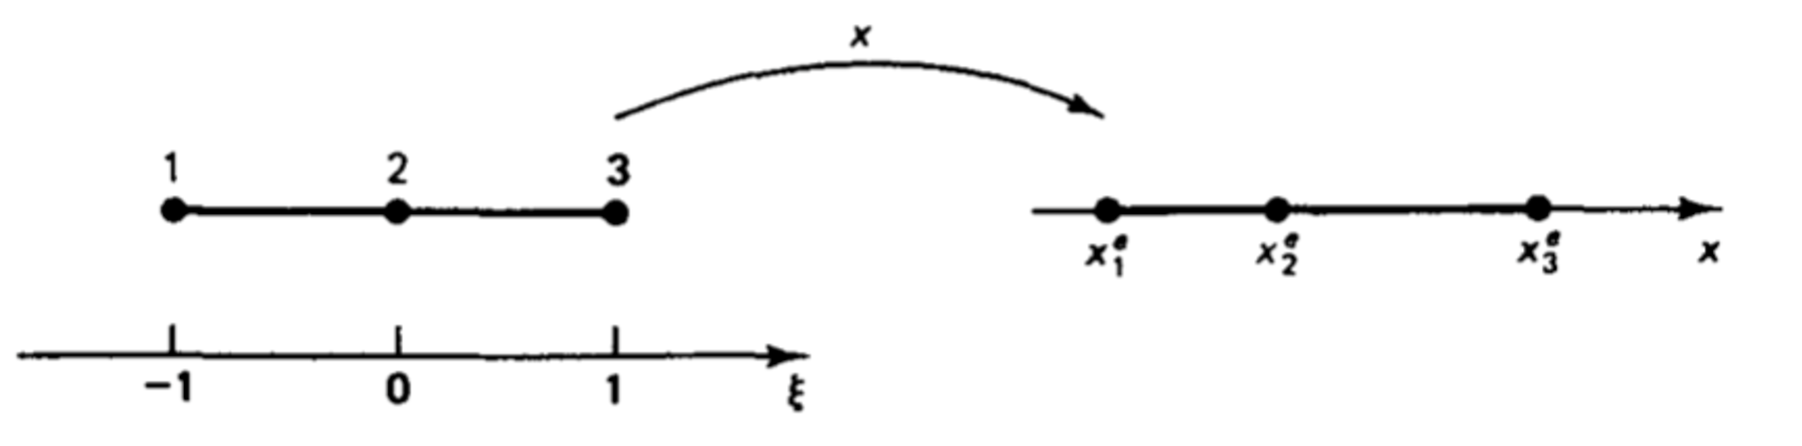
\includegraphics[angle=0, trim=0 0 0 0, clip=true, scale = 0.35]{./quad-elem.pdf}
\end{tabular}
\end{center} 
\caption{Quadratic element.}
\label{fig:quad_elem}
\end{figure}
\begin{enumerate}

\item Assume $f$ is constant and let $x_2^e = (x_1^e + x_3^e)/2$. Determine the exact expression for 
\begin{align*}
f_a^e=\int_{x_1^e}^{x_3^e} N_a f dx, \quad a = 1, 2, 3.
\end{align*}

\item Assume $f$ is constant, but make no assumption on the location of $x_2^e$ other than $x_1^e < x_2^e < x_3^e$. Determine the lowest-order Gaussian quadrature formula which exactly integrates $f^e$, and why?

\item Assume $x_2^e = (x_1^e + x_3^e)/2$. Determine the lowest-order quadrature formula for the element stiffness matrix, and why?

\item Modify the MATLAB code developed in class by using the quadratic three-node element, with the assumption that $x_2^e = (x_1^e + x_3^e)/2$.

\item Let the manufactured solution be $u = \sin(x)$. Design the source term and the boundary conditions. Perform calculations with equally spaced nodes for $4, 6, 8, 12$ and $16$ elements. 

\item Let $e := u^h - u$ be the error in the finite element approximation. Calculate
\begin{align*}
|e|_1 := \left( \int_0^1 \left( e_{,x} \right)^2 dx \right)^{\frac12},
\end{align*}
and 
\begin{align*}
|u|_1 := \left( \int_0^1 \left( u_{,x} \right)^2 dx \right)^{\frac12},
\end{align*}
plot $\log\left( |e|_1 /  |u|_1 \right)$ versus $\log(h) = - \log(n_{en})$. What is the slope of the curve?
\end{enumerate}
\end{enumerate}

\end{document}

